\section{Product Perspective}
The traditional application of an LMS is in educational institutions. Learning management systems have been used for several years to deliver courseware in schools and popularize e-learning. In the last few decades, Institutes have been using learning management systems to deliver training to internal employees and students. The LMS has become a powerful tool for staffing and training, extension schools, and any corporation looking to get a better grasp on the continuing education of its workforce. Its impact has been felt mostly outside of traditional education institutions, though the same technological and market forces are dramatically changing today’s classroom as well. \\

\noindent The Elearning system provides all vital information about institute such as all teachers, departments, students, list of events of respective institute in a systematic and user friendly manner. The student can see all his/her classmates and the teacher teaching the particular. The teachers can upload the assignments and quizes to his/her class and also can give marks according to the assignment submitted. On the other hand the student can see the notifications for important tasks also student can view the grades given to him by teacher as well as the quiz scorecard on the dashboard. The system also provides a special option called backpack where the student can save all the important stuff that is on his/her dashboard. Also there is a chat facility by which student and teacher can send each other personal message. Elearning systems are quite popular and useful these days, more and more institutes are implementing these systems. This system is also made to automate and easily manage the daily class work by reducing the use of pen and paper and thus saving a lot of time and money.



\section{Product Functions}
\begin{description}
\item[\bf{Registeration \& Login}:]
The software user would be required to Register through a screen. After 
authentication and login he would be able to access only those areas 
for which he is capable to access.
\item[\bf{Administrator Maintenance}:]
Administrator can add or update the details directly through admin 
interface.
\item[\bf{Add Class/Student}:]
New class and students can be added by the teacher.
\item[\bf{Class Calender}:]
Now the teachers and students can view the important event dates through the class calender.
\item[\bf{View Grades}:]
Students can view their result of quizes attempted and assignment grades from their portal.
\item[\bf{Change Avatar/Password}:] 
Both the teachers and student can change their password as well as avatar from their respective panels.
\item[\bf{Add Student}:] 
Teacher can add new student to his class.
\item[\bf{Send Message}:] 
Both the teacher and student can communicate with each other with the messaging facility.
\item[\bf{Upload/Submit Assignment}:] 
Using this function teacher can upload an assignment to his/her class, on the other hand the student can submit the assignment for evaluation.
\end{description}

\section{User Characteristics}
The objective of this elearning system is to provide an efficient and effective service to the students and teachers of any institute. It is aimed to encourage people to use computers and internet for their daily class work. Students can submit assignments online and or contact any student of their class by using the message facility provided in the system . Teachers can get status of a student's work.
The website has unique facility for uploading the content like assignments or any type of quiz along with the facility of backpack. This would help the students and teachers to reduce the use of pen and paper thus this will save a lot of time and money.
The students and teachers are the most expected users of this website,
but any person who is seeking information for is also a user.

\section{Constraints}
These constraints are given a constraint name and the DBA stores the constraints will its name and instruction internally along with the cell itself. If the data constraints attached to a specific cell in a table reference the contents of another cell in the table then the user will have to use table level constraint. Table level constraints are stored as a part of the global table definition. Constraints types:
\begin{itemize}
\item Null/Not Null
\item Unique
\item Primary Key
\item Foreign Key
\end{itemize}
\vspace{.5mm}
\begin{enumerate}
\item The Not Null Constraint: This ensures that null values are not permitted for the column; they serve as keys for operations on the table. Columns without the not null constraint allow null values. Not null is one of several integrity constraints that may be deined for table.
\item Unique Constraint: This designates a column or combination of columns as a unique key. No two rows in the table can have same value for this key. Null are allowed if the unique key is used on a single column. A column with this constraint will not accept any duplicate values.
\item Primary Key Constraint: As with unique key a primary key enforces uniqueness of the column combination involved and unique index is create to manage this. There may however be only one primary key in a table and this is known as definitive key through which rows in the table are individually identified. NULLS are not allowed primary key column. The LONG data types can not be included in a Primary key. A Primary key can contain 16 columns at most. A unique index is created on the column contained in the Primary key.
\item Foreign Key Constraint: Foreign keys representation relationships between tables. A foreign key is a column whose values are derived from the primary key of the same or same other table. The existing system of a foreign key implies that the table with foreign key is required to the primary key table from which the foreign key derived. A foreign key must have a corresponding primary key value n the primary key table to have a meaning.
\end{enumerate}

\section{System Design} Systems design is the process or art of defining 
the architecture, components, modules, interfaces, and data for a 
system to satisfy specified requirements. One could see it as the 
application of systems theory to product development. There is some 
overlap with the disciplines of systems analysis, systems architecture 
and systems engineering.
\begin{itemize}
\item  External design: External design consists of conceiving, 
planning out and specifying the externally observable characteristics 
of the software product. These characteristics include user displays 
or user interface forms and the report formats, external data sources 
and the functional characteristics, performance requirements etc. 
External design begins during the analysis phase
and continues into the design phase.
\item  Logical design: The logical design of a system pertains to an 
abstract representation of the data flows, inputs and outputs of the 
system. This is often conducted via modeling, which involves a 
simplistic (and sometimes graphical) representation of an actual 
system. In the context of systems design, modeling can undertake the 
following forms, including:
\begin{itemize}
\item Data flow diagrams
\item Entity Relationship Diagrams
\end{itemize}
\item  Physical design: The physical design relates to the actual 
input and output processes of the system. This is laid down in terms 
of how data is input into a system, how it is verified/authenticated, 
how it is processed, and how it is displayed as output.
\end{itemize}
\newpage
\section{Design Notations}
{\bf Data Flow diagrams}:
\image{0.5}{images/sss1.png}{DFD Notation}\\
{\bf Flow Charts}:
\image{0.5}{images/sss2.png}{Flow Chart Notations}\\
%Entity Relationship Diagrams:
%\image{0.6}{images/sss3.png}{ER Diagram Notation}\\
{\centering \bf Detailed Design}
We basically describe the functionality of the system internally. 
The internal design describes how data is flowing from database to the 
user and how they both are internally connected. For this reason we 
can show the design of the system in detailed manner by many ways: 
\section{Flowchart} 
A flowchart is a type of diagram that represents an
algorithm or process, showing the steps as boxes of various kinds, and
their order by connecting them with arrows. This diagrammatic
representation can give a step-by-step solution to a given problem.
Process operations are represented in these boxes, and arrows
connecting them represent flow of control. Data flows are not
typically represented in a flowchart, in contrast with data flow
diagrams; rather, they are implied by the sequencing of operations.
Flowcharts are used in analyzing, designing, documenting or managing a
process or program in various fields.
\image{0.67}{images/registration.png}{Flow Chart For Registration}
%\begin{figure}[ht]
%\centering
%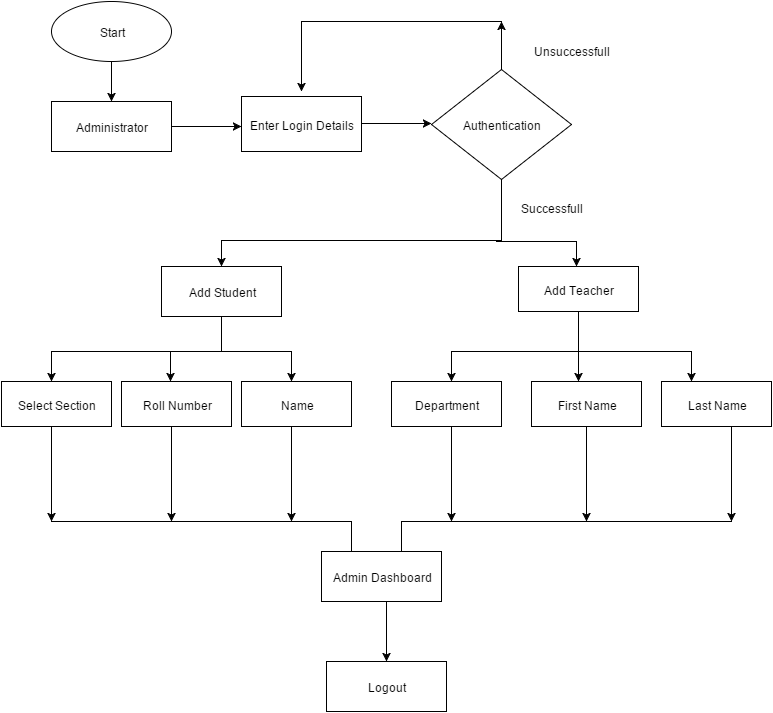
\includegraphics[scale=0.6]{images/addnew.png}
%\caption{Flow Chart For Adding New Teacher/Student}
%\end{figure}
\newpage
\image{0.5}{images/software.png}{Flow Chart For Working of System}
\newpage
\image{0.6}{images/addnew.png}{Flow Chart For Adding New Teacher/Student}

\newpage
\section{Database Design}
\image{0.4}{images/database.png}{Database Design}
\newpage
\section{Assumptions and Dependencies}
\subsection{Assumptions}
For Elearning System, main assumption was that this website may be viewed and even operated by literate person. Viewing the website is different than managing it. However it was not recommended to give access to uneducated people, but as the requirements specified by the client, the website must be designed in such a way that it should be so easy to manage that everyone can work on that.
\subsection{Dependencies}
However as such there is not any serious dependency of this system, but for viewer, it is recommended to it on modern browsers like FireFox and Google Chrome. However it also works with older browsers even with Internet Explorer. For user, it requires a Linux server. However it will also work on windows server if a WAMP/XAMPP server is installed.
As there is not hardware dependency of this website, i.e. it is viewable on all type of devices.
